\documentclass[12pt, twoside]{article}
\documentclass[12pt, twoside]{article}
\usepackage[letterpaper, margin=1in, headsep=0.2in]{geometry}
\setlength{\headheight}{0.6in}
%\usepackage[english]{babel}
\usepackage[utf8]{inputenc}
\usepackage{microtype}
\usepackage{amsmath}
\usepackage{amssymb}
%\usepackage{amsfonts}
\usepackage{siunitx} %units in math. eg 20\milli\meter
\usepackage{yhmath} % for arcs, overparenth command
\usepackage{tikz} %graphics
\usetikzlibrary{quotes, angles}
\usepackage{graphicx} %consider setting \graphicspath{{images/}}
\usepackage{parskip} %no paragraph indent
\usepackage{enumitem}
\usepackage{multicol}
\usepackage{venndiagram}

\usepackage{fancyhdr}
\pagestyle{fancy}
\fancyhf{}
\renewcommand{\headrulewidth}{0pt} % disable the underline of the header
\raggedbottom
\hfuzz=2mm %suppresses overfull box warnings

\usepackage{hyperref}
\usepackage{float}

\title{Algebra 2}
\author{Chris Huson}
\date{December 2023}

%\fancyhead[LE]{\thepage}
\fancyhead[RO]{\thepage \\ Name: \hspace{4cm} \,\\}
\fancyhead[LO]{BECA / Huson / Algebra 2: Polynomials \\* 13 December 2023}

\begin{document}

\subsubsection*{2.22 Do Now Quiz: Sequences, polynomials, exam review}
\begin{enumerate}

\subsubsection*{A2-APR.1 Perform operations with polynomials}
\item Find the sum in standard form $(4x^4+5x^3+3x^2-4) + (x^4-2x^3-2x^2-x+1)$. \vspace{3cm}

\subsubsection*{A2-F.IF.7c Graph polynomials, identify zeros, end behavior}
\item The polynomial $f(x)$ and linear function $g(x)$ are graphed below. 
\begin{multicols}{2}
    \begin{enumerate}[itemsep=0.6cm]
        \item What is the degree of $f(x)$?
        \item Is the leading coefficient of $f(x)$ positive, negative, or zero?
        \item If the polynomial $f(x)$ is written as the product of linear factors, what factor would be squared?
        \item Write down the three solutions to $f(x)=g(x)$ as ordered pairs.
    \end{enumerate} \vspace{1cm} \;

    \columnbreak

    \begin{tikzpicture}[xscale=0.7, yscale=0.7]
        \draw[lightgray,very thin] (-4,-2) grid (4,10);
        \draw [thick, ->] (-4.2,0) -- (4.4,0) node [above] {$x$};
        \draw [thick, ->] (0,-2.2)--(0,10.5) node [right] {$y$};
        \foreach \x in {-4,4} \draw (\x cm,5pt)--(\x cm,-5pt)node[below]{$\x$};
        \foreach \y in {-1,5,10} \draw (5pt,\y cm)--(-5pt,\y cm)node[left]{$\y$};
        \draw [thick, <->,smooth,samples=20,domain=3.15:-3.6] plot(\x,{-0.5*(\x-3)*(\x+2)^2})node[right]{\footnotesize $f(x)$};
        \draw [thick, <->,smooth,samples=20,domain=3.7:-3.7] plot(\x,{-0.5*(\x)+1.5})node[below left]{\footnotesize $g(x)$};
    \end{tikzpicture}
\end{multicols}

\subsubsection*{A2-F.BF.2 Write arithmetic and geometric sequences with recursive formulas}
\item Write a recursive definition of the sequence $a_1 = 4$, $a_2 = 12$, $a_3 = 36$, $a_4 = 108, \ldots$

\end{enumerate}
\end{document}